\section{Hydrostatik}
\subsection{Der Hydrostatische Druck \texorpdfstring{$p$}{p}}
\begin{bsp*}[ note = Flüssigkeit ]
	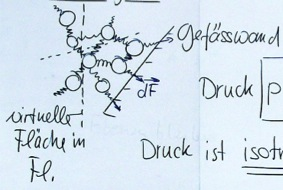
\includegraphics{Bild55} \\
	\[
		\text{Druck } p = \frac{\sum \dd F}{A}  \\
		[ p ] = \si{\newton\per\metre\squared}
	\]
	Druck ist isotrop!
\end{bsp*}

\subsection{Der Luftdruck (Gase)}
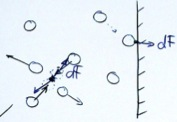
\includegraphics{Bild56}

\subsubsection{Experiment: Bierglas}
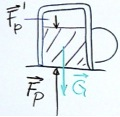
\includegraphics{Bild57}

\subsubsection{Magdeburger Halbkugeln}
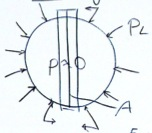
\includegraphics{Bild58}
\[
	p_L \approx 1 \text{bar} = 10^5 \text{Pa} \\
	A \approx 100 \text{cm}^2 \\
	F = p_L \cdot A = 10^3 \text{N} \approx 100 \text{kg}
\]

\begin{bsp*}[ note = Dehnung eines Blutgefässes ]
	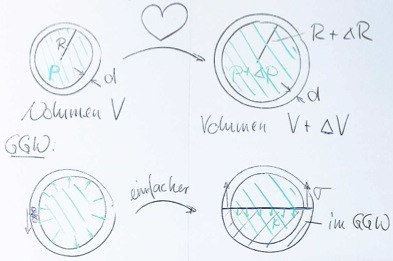
\includegraphics{Bild59} \\
	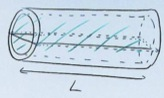
\includegraphics{Bild60}
	\[
		\underbrace{p \cdot 2 \cdot R \cdot L}_{\color{Red}\downarrow\downarrow\downarrow} = \underbrace{2 \cdot \sigma \cdot d \cdot L}_{\color{Blue}\uparrow\uparrow} \\
		\implies \text{ Spannung } \sigma = \frac{R}{d} \cdot p \text{ mit } \epsilon = \frac{\sigma}{E} \\
		\implies V \text{ nimmt zu} \\
		\vdots \\
		\frac{\Delta V}{V} = \frac{2 \cdot R}{E \cdot d} \cdot \Delta p \eqqcolon \overbrace{D}^{\text{Dehnbarkeit}} \cdot \Delta p
	\]
\end{bsp*}

Physiologie oft:
\[
	\frac{\Delta V}{V} = \frac{\Delta p}{\underbrace{k}_{\text{Volumenelastizitätsmodul}}} \\
	k = \frac{1}{D}
\]

\subsubsection{Aneurysma}
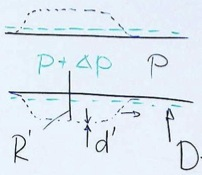
\includegraphics{Bild61}
\[
	D = \frac{2R}{Ed} \\
	D' = \frac{2R'}{Ed'} > D \\
	\text{altendes Blutgefäss } E \nearrow \implies D \searrow
\]
$\implies$ krakhafte Gefässerweiterung

\begin{rep*}[ note = Hydrostatik ]
	hydrostatischer Druck in Flüssigkeiten / Gasen:
	\[ p = \frac{\sum \dd F}{A} \]
	\begin{itemize}
		\item isotrop!
		\item Luftdruck $p_0$
			\[ p_0 \approx 10^5 \text{Pa} = 1 \text{bar} \corresponds 1 \frac{\text{kg}}{\text{cm}^2} \text{!} \]
	\end{itemize}
	\begin{bsp*}[ note = Dehnung eines Gefässes ]
		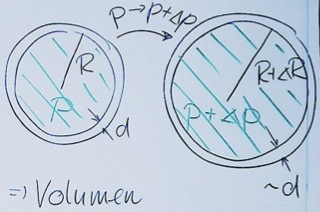
\includegraphics{Bild62} \\
		$\implies$ Volumen
		\[
			V \rightarrow V + \Delta V \\
			\frac{\Delta V}{V} = \underbrace{\frac{2R}{Ed}}_{\text{Dehnbarkeit}} \cdot \Delta p
		\]
	\end{bsp*}
\end{rep*}

\subsubsection{Druckverteilung in Flüssigkeiten}
(auf Erdoberfläche) \\
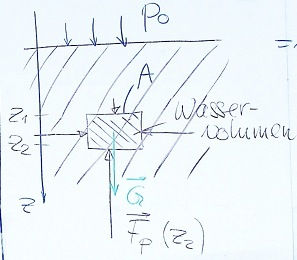
\includegraphics{Bild63} \\
GGW
\[
	F_p( z_1 ) + G = F_p( z_2 ) \\
	F_p( = p \cdot A \\
	\implies p( z_2 ) = p( z_1 ) + \frac{G}{A} \\
	\implies p( z_2 ) = p( z_1 ) + \frac{( z_2 - z_1 ) \cdot \cancel{A} \cdot \rho \cdot g}{\cancel{A}} \\
	\text{Wähle } z_1 = 0 , z_2 = z \\
	p(z) = p_0 + z \cdot \rho \cdot g
\]

10m Wassertiefe
\[
	\rho \cdot g \cdot z = 10^3 \frac{\text{kg}}{\text{m}^3} \cdot 10 \frac{\text{m}}{\text{s}^2} \cdot 10 \text{m} = 10^5 \text{Pa} = 1 \text{bar} \\
	1 \text{mm} \ce{H20} \implies p = 9.8 \text{Pa} \\
	1 \text{mm} \ce{Hg} \implies p = 133 \text{Pa} \eqqcolon 1 \text{torr} \\
	\text{Blutdruck } \overline{p} \approx 100 \text{mm \ce{Hg}} = 133 \text{mbar}
\]

\subsubsection{Atmung beim Tauchen}
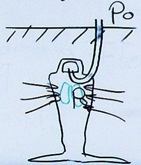
\includegraphics{Bild64}

\subsubsection{Luftdruck}
\[
	p_L(z) = ? \\
	\rho_L \approx 1 \frac{\text{kg}}{\text{m}^3} \\
	\rho_W \approx 10^3 \frac{\text{kg}}{\text{m}^3}
\]

\subsection{Der Auftrieb}
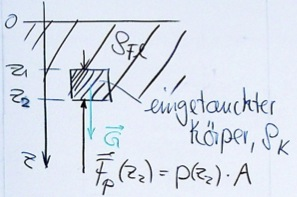
\includegraphics{Bild65}
\[
	F_{\text{res}} = F_p(z_1) + G - F_p(z_e) = G - ( p(z_2) - p(z_1) ) \cdot A = ( z_2 - z_1 ) A \cdot \rho_K \cdot g \underbrace{ - ( z_2 - z_1 ) A \cdot g \cdot \rho_{\text{Fl}}}_{F_A} \\
	F_{\text{res}} = \underbrace{( z_2 - z_1 )}_{V_K} \cdot A \cdot g ( \rho_K - \rho_{\text{Fl}} \\
	\rho_K > \rho_{\text{Fl}} = F_{\text{res}} > 0 \quad \downarrow \\
	\rho_K < \rho_{\text{Fl}} = F_{\text{res}} < 0 \quad \uparrow
\]

\subsubsection{Druckverteilung in Zentrifuge}
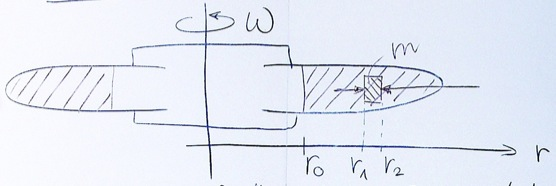
\includegraphics{Bild66} \\
$\implies$ Trennung von Stoffen durch Sedimentation $m$ auf Kreisbahn $\implies$ Zentripetalbeschleunigung $a_z$
\[
	a_z = \frac{v^2}{r} = r \omega^2
	\intertext{2.N.P $F_z = m a_z$ ; Rechnung:}
	\dots p(r) = p_0 + \frac{1}{2} \rho_{\text{Fl}} \omega^2 (r^2 - r_0^2)
	\intertext{Ultrazentrifuge 100000 $\frac{\text{U}}{\text{min}}$}
	\omega = 2\pi f = 10500 \text{s}^{-1} \\
	r \approx 5 \text{cm} \\
	\implies p \approx 1.3 \text{kbar}
\]
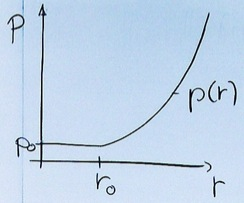
\includegraphics{Bild67}
